%----------------------------------------------------------------------------
\chapter{Bevezetés}
%----------------------------------------------------------------------------
	1986-ban Binning demonstrálta az atomerő mikroszkóp (AFM) ötletét \cite{Binnig1986}, ami mára 
	a nanotechnológia egyik legfontosabb eszköze képalkotásra használható képalkotásra, nanolitográfiára és 
	adott anyag alakítására \cite{Vasic2013}.
	Az AFM apparátusa az adott minta felületé és pásztázó kantilever végére erősített tű 
	kölcsönhatásának vizsgálatát végzi. (lásd \ref{fig:tip-sample}. ábra)
	A felület és a tű közötti domináns kölcsönhatás határozza meg, hogy az anyag melyik fizikai
	mennyiségét kaphatjuk meg.
	\begin{figure}[H]
		\centering
		\subfloat[Az AFM apparátusa]{
			\includegraphics[width=0.4\columnwidth]{figures/eps/AFM.eps}%
			\label{fig:afm}
		}
		\hfil
		\subfloat[A tű és minta modellje]{
			\includegraphics[width=0.4\columnwidth]{figures/eps/tip-sample.eps}
			\label{fig:tip-sample}
		}
		\caption{Az AFM apparátusa látható az (a) ábrán. A lázernyaláb
		a tű felületéről tükröződve egy fotódetektorra irányul. A tű pozícióját ez alapján nagy pontossággal ismerjük. A
		(b) ábrán a minta és a felette lévő tű modellje látható a kapacitás analitikus számításához.
		A tű $R$ sugarú $H$ magasságú és $D$ távolságra van a mintától. (Forrás: \cite{Butt20051})}
		\label{fig:fig_sim}
	\end{figure}
	Az AFM felhasználása kontakt illetve kopogtató üzemmódú lehet. A kontakt mód során a
	felületen végighúzzuk a tűt és mérjük a $z$ irányú elmozdulását. Így képesek vagyunk a minta
	felületén lévő atomok elrendezéséről magasságtérképet adni.
	Kopogtató mód \cite{Martin1987} során a tűt elemeljük a mintától és $f$ frekvenciával rezegtetjük.
	A letapogatás során az  átlagos minta-tű távolságot a kontakt módú magasságtérkép felhasználásával
	konstans értéken tartjuk.
	A kantilever dinamikáját ismerve a rezegtetés frekvenciájának eltéréséből
	számítható a tűre ható erő. Ezen erő nagyságát befolyásoló tényezők:
	\begin{enumerate}[a)]
		\item a minta és a tű kapacitására kapcsolt feszültség,\label{cap_force}
		\item a minta felületi töltéssűrűség eloszlása,\label{sc_force}
		\item Van der Waals erő.\label{vdw_force}
	\end{enumerate}
	A dolgozatban a felületi töltéssűrűség mérését tekintem célnak.
	
	A \cite{Butt1991Dec, Butt20051} szerint az erő \ref{cap_force} komponensét a minta és a tű közötti
	kapacitásból az \eqref{eq:capforce} szerint származtathatjuk.
	\begin{equation}\label{eq:capforce} 
	F_{s} = -\frac{\ud E}{\ud D} = -\frac{\ud (CV^2 /2)}{\ud D} = -\frac12 \frac{\ud C}{\ud D} V^2   
	\end{equation}
	Ha a minta pásztázása során ezen \ref{cap_force} erőkomponens konstansnak mondható, tehát a felületi
	érdesség és a távolság pontatlansága elhanyagolhatóan kicsi, akkor a töltéssűrűség mérésében ez állandó hibát okoz. ami
	eliminálható.
	Az \eqref{eq:capforce} számításában a kritikus elem a kapacitás értéke, amit numerikus számítás
	mellőzése esetén a \cite{Hudlet1998} szerinti analitikus eredményt használhatjuk fel.
	A tű formáját a \ref{fig:tip-sample} ábra szerintinek veszi és a mintát sík felületnek feltételezi.
	A tűre vonatkozó feltételezés legtöbb esetben helyénvaló, viszont a minta nagyfokú érdessége és változatossága végett érvényét
	veszti. Szemléltetését a \ref{fig:terkep_anim} ábrán lehet látni. 
	Ilyen esetben a kapacitás értéke mintáról mintára változik és állandó hiba helyett, a mérést zajként terheli.
	\begin{center}
		Ezen zaj kiküszöbölése a kapacitás numerikus szimulációjával lehetséges.
	\end{center}
	A probléma ezzel, hogy ezen szimulációt minden egyes mérési pontban el kell végezni, aminek a kivitelezése
	csak multiprocesszoros környezetben lehetséges elfogadható idő alatt.
	
	\begin{figure}[!hp]
		\begin{center}
		\subfloat[1. pillanat]{
			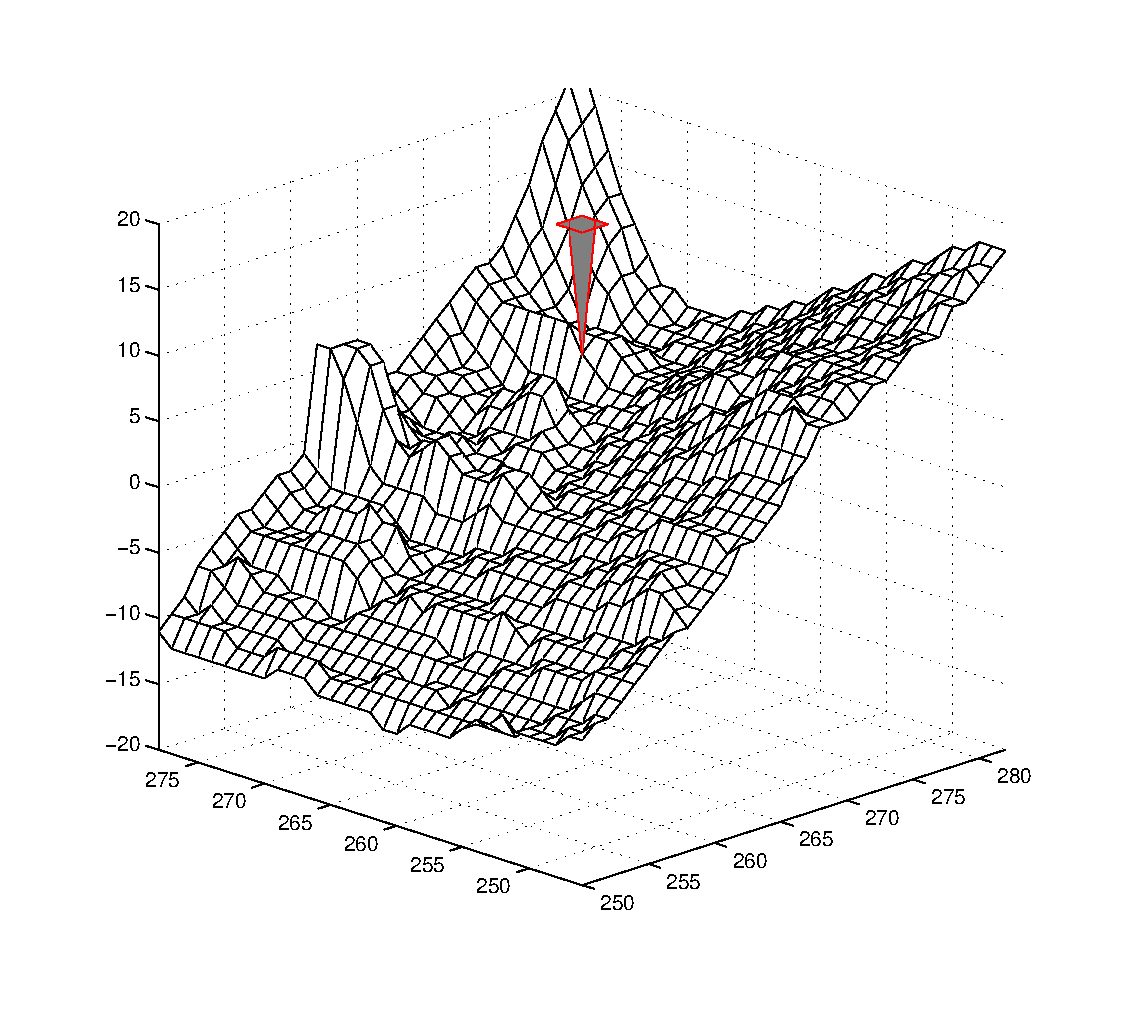
\includegraphics[height=0.22\paperheight]{figures/eps/el_1.eps}%
			%\label{fig:afm}
		}\\
		\subfloat[2. pillanat]{
			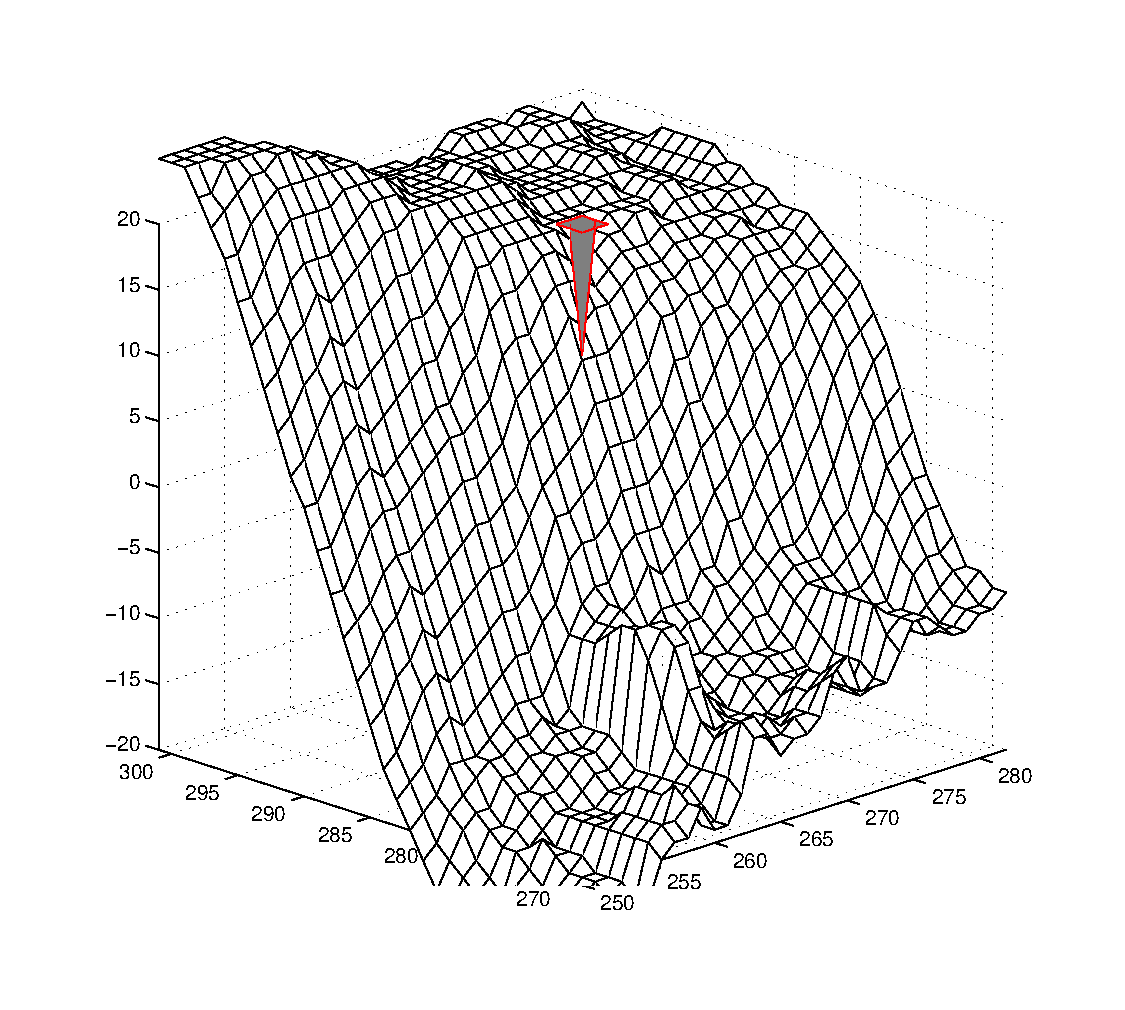
\includegraphics[height=0.22\paperheight]{figures/eps/el_2.eps}%
			%\label{fig:afm}
		}\\
		\subfloat[3. pillanat]{
			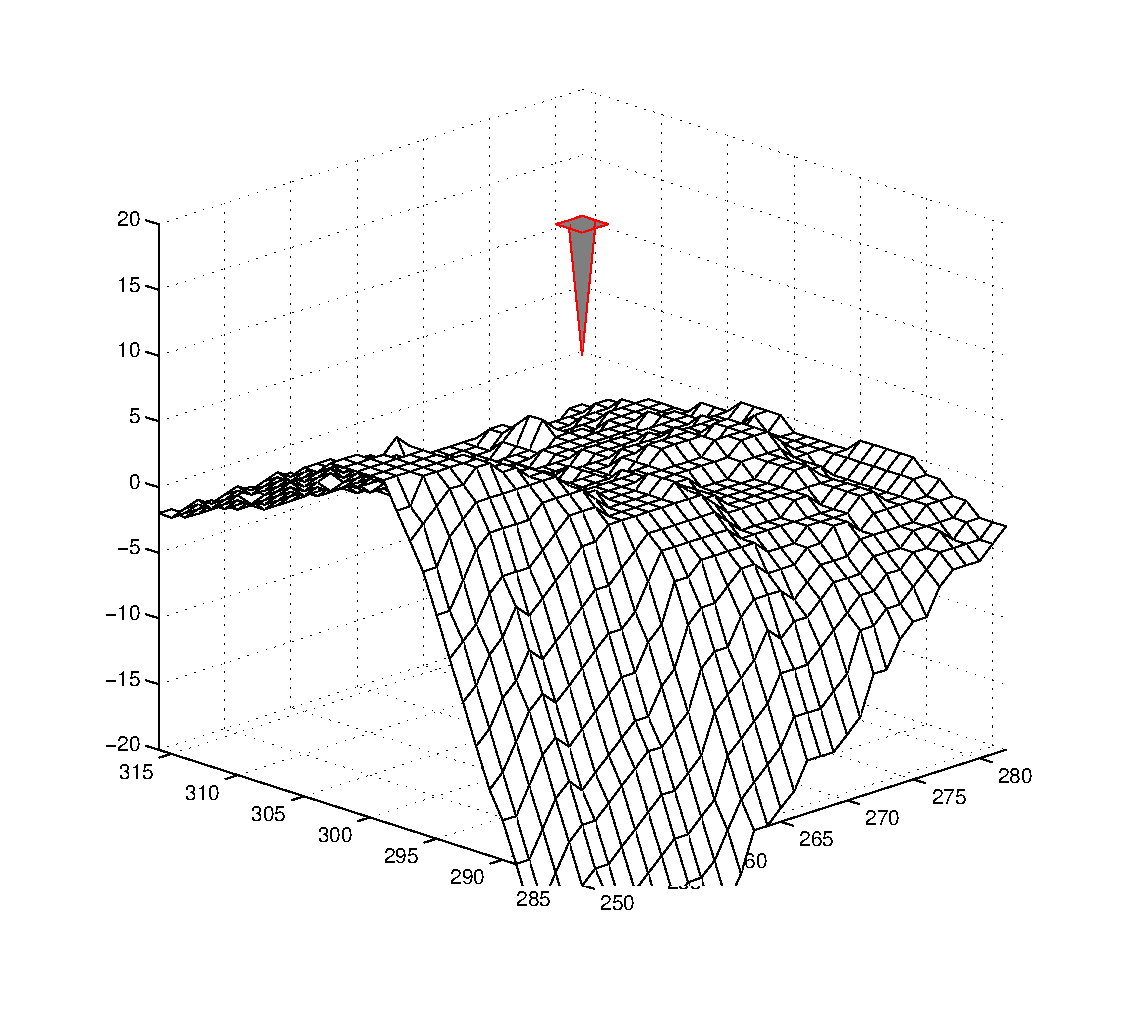
\includegraphics[height=0.22\paperheight]{figures/eps/el_3.eps}%
			%\label{fig:afm}
		}\\
		\caption{A magasságtérkép változása a második mérés során fix pozíciójú tű esetén.}
		\label{fig:terkep_anim}
		\end{center}
	\end{figure}